%!TEX root = uw-ethesis.tex
% chktex-file 46 (ignore warnings about $...$)
% chktex-file 24 (ignore \label warning)
% chktex-file 35  (disables warning for {max/min})
\renewcommand{\L}{\mathcal{L}}
\chapter{Introduction}\label{chap:intro}

%%%%%%%%%%%%%%%%%%%%%%%%%%%%%%%%%%%%%%%%%%%%%%%%%%%%%%%%%%%%%%%%%%%%%%%%%%%%%%%%
%%%%%%%%%%%%%%%%%%%%%%%%%%%%%%%%%%%%%%%%%%%%%%%%%%%%%%%%%%%%%%%%%%%%%%%%%%%%%%%%
\section{Motion Planning}
%%%%%%%%%%%%%%%%%%%%%%%%%%%%%%%%%%%%%%%%%%%%%%%%%%%%%%%%%%%%%%%%%%%%%%%%%%%%%%%%
%%%%%%%%%%%%%%%%%%%%%%%%%%%%%%%%%%%%%%%%%%%%%%%%%%%%%%%%%%%%%%%%%%%%%%%%%%%%%%%%

Planning is a fundamental problem in robotics: mobile robots must be able to determine how to move in order to perform tasks. According to LaValle in his titular book on planning algorithms, converting high-level specifications into low-level descriptions of how a robot ought to move is what is generally referred to as motion planning~\cite{LaValle2006}. He further states motion planning, in modern control theory literature, refers to the generation of inputs to a dynamical system which drive it from an initial state to a specified goal state (or set).

In general, motion planning solves problems involving a \emph{state space}, which is the set of all possible states in which a system could find itself. Such a space could be finite, like in the case of Rubik's cube with finitely many configurations, or infinite, such as train with both a position and velocity that can vary continuously in the domain of real numbers. Note that \emph{time} also plays a crucial role in both of these examples: the Rubik's cube allows moves in succession, in some order, and the train's location and current velocity depend on its past position and velocity. Lastly, in order to plan, one must be able to affect the system, i.e., change the state, in the some way. Some systems, like the train, abide by a set of dynamics which govern how the system changes. A train on a steep hill will roll down the hill if it does not have sufficient momentum to crest over the top. However, if we allow the system to accept an \emph{input} or \emph{control}, then the system can be altered to act in a desirable way. Being able to set the engine to full-throttle may make the difference between getting to the destination and ending up stuck at the foot of the hill. For continuous time systems, the dynamics are modeled with ordinary differential equations. Even for systems without dynamics, like with the Rubik's cube (assuming we are not concerned with how the faces of the cube are rotated), there must be a way to specify exactly how an action affects the state of the system.

This thesis will focus only on continuous-time motion planning problems, where the dynamics are modeled by a control system consists of a set of ordinary differential equations modeling the dynamic of the system, an initial condition, a set of allowed states, and a set of admissible controls. Note that this does not rule out the possibility of uncertainties. Dynamical systems model reality but do not necessarily do so with complete accuracy, and disturbances in the environment may also have an effect on the behaviour of a system. A well-designed motion planning algorithm can help to reject disturbances and be robust under uncertainties.


%%%%%%%%%%%%%%%%%%%%%%%%%%%%%%%%%%%%%%%%%%%%%%%%%%%%%%%%%%%%%%%%%%%%%%%%%%%%%%%%

\subsection{Examples}

Motion planning has an immense variety of applications in both virtual and robotic systems. Moreover, the potential for autonomous robots to improve human living conditions is vast, and as yet not fully understood. One especially disruptive emerging technology is autonomous vehicles: cars and trucks that are able to drive from an initial position to a goal location with minimal or no human input~\cite{Thrun2010}. These autonomous vehicles have been gaining popularity in recent years, especially with the media hype of Google and Tesla bringing self-driving cars into the public eye; however, the first research on this topic began in the 20th century. By 1995, Todd Jochem and Dean Pomerleau completed a 2,797 mile journey across America in a van using neural networks to design a vision-based partially automated driving system\footnote{The trip was titled ``No Hands Across America'' since the only human input involved braking and accelerating; steering was performed completely autonomously.}~\cite{Jochem}. This accomplishment demonstrated level 2 automation under the SAE International Standard J3106~\cite{SAEinternational2016}, which falls short of being described as an ``automated driving system'' as a human driver is still essential. More recent advances have brought autonomous vehicles to level 3 with Google's self-driving car having over 500,000 miles of autonomous driving in 2012~\cite{Lutin2013}. Level 3 is labeled as ``conditional automation'', meaning for certain driving modes the automated driving system can control all aspects of driving with the caveat that a human driver be on standby to respond to requests to intervene. In jumping from level 2 to level 3, a human driver becomes non-essential to the driving task, except as a fallback.

Another practical example of motion planning is controlling an \gls{uav} system, such as a quadrotor. Due to their scalable size and high maneuverability, quadrotors are used for an ever-increasing range of tasks, from aerial photography, to mapping dangerous, cluttered, or unexplored regions with \gls{slam}, to light shows from a fleet of Intel's quadrotors, and even for quickly delivering small parcels~\cite{Yang2013, Richter2016}. Each of these tasks requires a means of determining where and how the quadrotor should move, and advances in motion planning will allow for even more complex and intricate maneuvers, and therefore more applications. However, planning for quadrotors can be quite difficult because, like cars, they are non-holonomic, and are therefore subject to differential constraints. Since they can maneuver in 3D space instead of being restricted to a 2D surface, as is the case for ground vehicles, quadrotors are described by a 12-dimensional state space (position, velocity, orientation, and rotational velocity). This often means that much computational effort is involved in motion planning for \gls{uav} systems. Furthermore, given that the dynamics governing quadrotor motion are highly nonlinear, motion planning is all the more difficult, from path generation to trajectory tracking. Many of these issues will be addressed in \autoref{chap:quad}, which presents a framework for real-time motion planning of quadrotors, based on work by Allen et al.~\cite{Allen2016}.

Overall, the field of robotics is continuing to grow, and with it, motion planning is becoming all the more relevant and important in day-to-day life. Forklifts are being automated to move merchandise around in warehouses, and vacuum cleaners have become small disks that roam around the home like robotic pets. In the field of agriculture, robots are improving the lives of farmers by autonomously targeting and removing weeds that negatively impact crops~\cite{Wendel2016}. The recurring theme in all of these examples is that automation, along with the essential component of motion planning, is leading the way in reducing the need for human labour. Robots are becoming increasingly capable of performing complex tasks, especially with the concurrent rise of machine learning and artificial intelligence, and advances in motion planning are leading to improved performance~\cite{Greeff2018}, online reactivity to dynamic obstacles~\cite{Allen2016}, and better guarantees~\cite{Lin2014} in all areas of robotics.


%%%%%%%%%%%%%%%%%%%%%%%%%%%%%%%%%%%%%%%%%%%%%%%%%%%%%%%%%%%%%%%%%%%%%%%%%%%%%%%%

\subsection{Sampling-Based Motion Planning}\label{intro:sbmp}

The sampling-based approach to motion planning has become particularly popular in robotics applications since it avoids having to explicitly define obstacles (dually, the free space). In essence, the strategy is to sample the state space in order to create a graph which explores a representative portion of the space. Such problems can be solved geometrically, meaning solutions only find a collision-free path in space and do not take into account feasibility, or using kinodynamic planning, which considers the system dynamics and differential constraints to ensure the robot can accomplish the planned task. In this thesis, emphasis is placed on kinodynamic planning.

The general approach to sampling-based motion planning begins with choosing a sampling scheme; that is, samples of the state space are to be taken either deterministically, or according to some probability distribution. These samples are then used to generate new nodes on a graph, where the details involved in connecting each new node to the existing graph vary based on the sampling-based algorithm being applied. For example, as depicted in \autoref{rrt}, the popular motion planning algorithm \gls{rrt} samples a random point in state space, finds the nearest existing point of the tree, and steers from said nearest point towards the sample up to some maximum distance, $\delta_{max}$. The result is a newly added edge (transition from one state to another) and node (state) in the tree. The fact that steering is required means there must exist a function which optimally connects two states. This requirement is is quite strict, and will be discussed in \autoref{chap:prelims} and \autoref{chap:sstpaper}.

\begin{figure}
    \begin{center}
        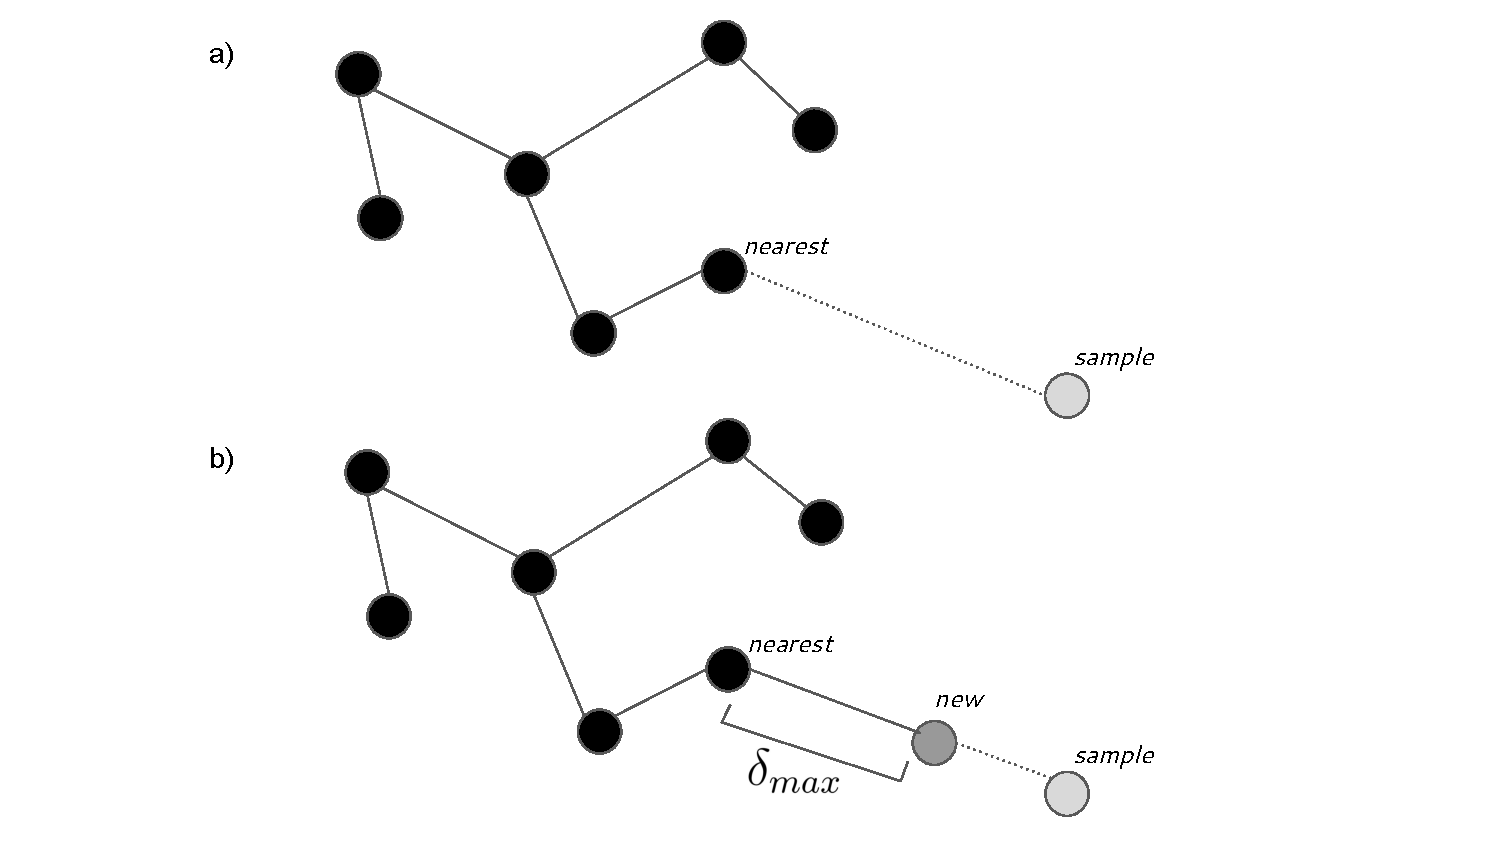
\includegraphics[width=\textwidth]{./figures/RRT_figure.pdf}
    \end{center}
    \caption[RRT sampling and connection procedure]{\gls{rrt} sampling and connection procedure. The existing tree is shown with black nodes and solid edges.\ $\text{a}\rparen$ A node is randomly sampled from the state space, and the nearest existing node is found.\ $\text{b}\rparen$ A new node and edge are added to the tree along the line connecting the nearest and sampled nodes, but at a maximum distance $\delta_{max}$ from the nearest node.}
\label{rrt}
\end{figure}

An important concept in motion planning literature is {\em completeness}, and we say that an algorithm is complete if, for any input, it correctly returns in finite time whether or not there exists a solution to the path planning problem~\cite{LaValle2006}. Clearly, due to the nature of sampling-based algorithms, completeness cannot be achieved. There are, however, weaker notions of completeness which can be useful to study. One common alternative when using a random sampling scheme is the the notion of {\em probabilistic completeness}, which means that the probability that the algorithm finds a solution (if one exists) converges to 1 as the number of samples tends to infinity. Similarly, we that a motion planning algorithm is {\em asymptotically\/optimal} if the probability of finding an optimal solution (based on a preestablished cost function) approaches $1$ as the number of samples approaches infinity~\cite{Karaman2011}.

% TODO: MORE



%%%%%%%%%%%%%%%%%%%%%%%%%%%%%%%%%%%%%%%%%%%%%%%%%%%%%%%%%%%%%%%%%%%%%%%%%%%%%%%%
%%%%%%%%%%%%%%%%%%%%%%%%%%%%%%%%%%%%%%%%%%%%%%%%%%%%%%%%%%%%%%%%%%%%%%%%%%%%%%%%
\section{Temporal Logic}
%%%%%%%%%%%%%%%%%%%%%%%%%%%%%%%%%%%%%%%%%%%%%%%%%%%%%%%%%%%%%%%%%%%%%%%%%%%%%%%%
%%%%%%%%%%%%%%%%%%%%%%%%%%%%%%%%%%%%%%%%%%%%%%%%%%%%%%%%%%%%%%%%%%%%%%%%%%%%%%%%


Motion planning occurs on various levels of abstraction. A hierarchical control structure would typically have some ``vague'', high-level description of what the robot or system is supposed to do at the top, guiding the desired behaviour. Below that there is a model, usually encompassing system dynamics, with a control architecture that prescribes how information is passed along in a series of inputs and outputs, which ultimately generates a motion plan to be followed. At the lowest levels, algorithms are used to put the motion plan in action, using a tracking controller (typically with some form of feedback to improve robustness) that determines exactly what inputs ought to be applied to maneuver along the planned path trajectory.

Temporal logics are the language used to express the high-level specifications that preside over the control hierarchy, dictating what the user desires. Most instances of motion planning seek simply to move from one location to another, without any other instructions (except to avoid obstacles). This goal is often hard-coded into the algorithms designed for solving motion planning problems. However, there exists a much broader world of possibility, and allowing users to specify exactly what is desired of a robot opens many avenues for real-world applications, not to mention the benefit of having performance guarantees from the use of formal methods~\cite{Lin2014}. We choose to work with \mucalc{} is a highly expressive temporal logic which permits more diverse and complex specifications than the most widely used temporal logics, including \gls{ltl}, \gls{ctl}, and extensions thereof~\cite{Karaman2009}, as well as for the relative ease and elegance of model checking that it permits. An in-depth background on \mucalc{} is provided \autoref{chap:prelims}.

% TODO: MORE?


%%%%%%%%%%%%%%%%%%%%%%%%%%%%%%%%%%%%%%%%%%%%%%%%%%%%%%%%%%%%%%%%%%%%%%%%%%%%%%%%
%%%%%%%%%%%%%%%%%%%%%%%%%%%%%%%%%%%%%%%%%%%%%%%%%%%%%%%%%%%%%%%%%%%%%%%%%%%%%%%%
\section{Contributions}
%%%%%%%%%%%%%%%%%%%%%%%%%%%%%%%%%%%%%%%%%%%%%%%%%%%%%%%%%%%%%%%%%%%%%%%%%%%%%%%%
%%%%%%%%%%%%%%%%%%%%%%%%%%%%%%%%%%%%%%%%%%%%%%%%%%%%%%%%%%%%%%%%%%%%%%%%%%%%%%%%

Summarizing the contributions of this thesis, we have successfully solved a kinodynamic planning problem with temporal logic specifications without the need for a solution to an \gls{obvp}, also called a steering function. While using temporal logic specifications with motion planning has been heavily researched, e.g.,~\cite{Ayala2013, Bhatia2010, Karaman2009,Lin2014, Wolff2014}, it is often difficult or impossible to find a steering function, allowing motion planning only for simple dynamical systems. Addressing this issue, we have developed a means of combining the asymptotically optimal and probabilistically complete kinodynamic planning algorithm \gls{sst}* (see \autoref{prelims:sst}) from~\cite{Li2016} with the model checking procedure from~\cite{Karaman2009} to create a motion planning algorithm with deterministic \mucalc{} specifications that does not rely on a steering function. By merging information obtained from multiple Kripke structures, we are able to create one \emph{abstracted Kripke structure} which stores the most cost-efficient paths that reach other proposition regions of the state space. To connect the trajectories found from multiple Kripke structures, an \gls{lqr} feedback control policy is used to track the candidate trajectories stored in the abstracted Kripke structure. Simulations demonstrate that it is possible to satisfy a complex liveness specification for infinitely often reaching three regions of state space using only forward propagation.

Furthermore, we use the notion of an abstracted Kripke structure to solve the planning problem with temporal logic specifications on the highly nonlinear quadrotor system. % TODO: abstract kripke + FMT

An introductory overview of \mucalc{} is conducted in \autoref{chap:prelims} which is intended to be both detailed and understandable. Many early papers on the subject are cited and amalgamated into one section to provide readers with a deep intuition on the subject of temporal logic using \mucalc{}. Deterministic \mucalc{} receives particular attention due to its impressive expressiveness coupled with its propensity for fast model checking.

We also provide many details and clarifying explanations that are missing from some of the key papers regarding quadrotor motion planning, including quadrotor dynamics~\cite{Mellinger2011}, real-time planning~\cite{Allen2016}, and geometric control methods~\cite{Lee2010}, in \autoref{chap:quad}. Much of the literature in this area focuses on the engineering aspects or provides too little (or convoluted) justification for results; in contrast, we take a deeper look at the mathematics involved in deriving many of the equations that arise in kinodynamic planning for quadrotors. Moreover, the provided level of detail should be sufficient in guiding the interested reader to implement the algorithms and frameworks discussed herein.


%%%%%%%%%%%%%%%%%%%%%%%%%%%%%%%%%%%%%%%%%%%%%%%%%%%%%%%%%%%%%%%%%%%%%%%%%%%%%%%%
%%%%%%%%%%%%%%%%%%%%%%%%%%%%%%%%%%%%%%%%%%%%%%%%%%%%%%%%%%%%%%%%%%%%%%%%%%%%%%%%
\section{Overview}
%%%%%%%%%%%%%%%%%%%%%%%%%%%%%%%%%%%%%%%%%%%%%%%%%%%%%%%%%%%%%%%%%%%%%%%%%%%%%%%%
%%%%%%%%%%%%%%%%%%%%%%%%%%%%%%%%%%%%%%%%%%%%%%%%%%%%%%%%%%%%%%%%%%%%%%%%%%%%%%%%

The rest of this thesis is structured as follows. \autoref{chap:prelims} introduces many of the important and recurring concepts discussed throughout. The syntax and semantics of \mucalc{} are provided, and a crucial theorem used in model checking is stated with proof. Then, the fragment of \mucalc{} we will use, called deterministic \mucalc{}, is defined. Lastly, many common specifications are described in detail to provide the foundations of the language of our temporal logic specifications. We then move to a description of the kinodynamic planning algorithm \gls{sst}* which we will use in \autoref{chap:sstpaper}. The final section of this chapter provides a detailed look at the \gls{fmt} algorithm, which we use for quadrotor motion planning.

The next chapter (\autoref{chap:sstpaper}) demonstrates novel research on solving kinodynamic planning problems while satisfying deterministic \mucalc{} specifications without requiring a steering function. A problem statement is provided along with a detailed description of the meta-algorithm \texttt{KinoSpecPlan} which combines using \gls{sst}* with a local deterministic model checking algorithm as well as \gls{lqr} tracking. A complex liveness specification is then shown to be satisfied in an example that uses this method.

\autoref{chap:quad} focuses on the application of kinodynamic planning to quadrotors. The dynamics of a quadrotor system are derived, and the problem of planning with deterministic \mucalc{} specifications is stated. We then outline all of the necessary components for a real-time motion planning framework and demonstrate some simulation results for the task of transiting from an initial state to a goal state. Lastly, the ideas from \autoref{chap:sstpaper} are used in the context of quadrotor planning to produce trajectories satisfying temporal logic specifications.
%TODO: has this last part changed?

Lastly, \autoref{chap:conc} offers closing remarks as well as directions for future work.
